\documentclass[aspectratio=169,10pt]{beamer}

% ---------- Theme: clean, technical, no cheesy defaults ----------
\usetheme{Madrid}
\usecolortheme{default}
\setbeamertemplate{navigation symbols}{}
\setbeamertemplate{footline}[frame number]
\setbeamercovered{transparent}

\definecolor{navy}{RGB}{30,39,97}
\definecolor{ice}{RGB}{202,220,252}
\definecolor{darktext}{RGB}{26,26,46}
\definecolor{muted}{RGB}{92,107,138}
\definecolor{accent}{RGB}{232,163,61}
\definecolor{cardbg}{RGB}{244,246,252}
\definecolor{goodgreen}{RGB}{30,122,70}
\definecolor{badred}{RGB}{192,57,43}

\setbeamercolor{structure}{fg=navy}
\setbeamercolor{title}{fg=white}
\setbeamercolor{frametitle}{fg=white,bg=navy}
\setbeamercolor{palette primary}{fg=white,bg=navy}
\setbeamercolor{palette secondary}{fg=white,bg=navy}
\setbeamercolor{palette tertiary}{fg=white,bg=navy}
\setbeamercolor{footline}{fg=muted,bg=white}
\setbeamerfont{frametitle}{series=\bfseries}

\usepackage[T1]{fontenc}
\usepackage{booktabs}
\usepackage{array}
\usepackage{tikz}
\usetikzlibrary{shapes.geometric,positioning,arrows.meta}
\usepackage{pgfplots}
\pgfplotsset{compat=1.18}
\usepackage{xcolor}
\usepackage{tcolorbox}
\tcbuselibrary{skins}

\newtcolorbox{cardbox}[1][]{colback=cardbg,colframe=cardbg,boxrule=0pt,arc=3pt,left=8pt,right=8pt,top=6pt,bottom=6pt,#1}
\newtcolorbox{navybox}[1][]{colback=navy,colframe=navy,coltext=white,boxrule=0pt,arc=3pt,left=8pt,right=8pt,top=6pt,bottom=6pt,#1}
\newtcolorbox{greenbox}[1][]{colback=goodgreen,colframe=goodgreen,coltext=white,boxrule=0pt,arc=3pt,left=8pt,right=8pt,top=6pt,bottom=6pt,#1}
\newtcolorbox{redbox}[1][]{colback=badred,colframe=badred,coltext=white,boxrule=0pt,arc=3pt,left=8pt,right=8pt,top=6pt,bottom=6pt,#1}

\title{\textbf{Quantum RNA Secondary Structure Prediction}}
\subtitle{Optimizing mRNA MFE folding with real thermodynamic energies, validated on D-Wave and IBM quantum hardware}
\author{Team Qudit Creons}
\institute{WISER 2026 --- Moderna Challenge}
\date{}

\begin{document}

% ============================================================ TITLE
{
\setbeamertemplate{footline}{}
\begin{frame}[plain]
  \begin{tikzpicture}[remember picture, overlay]
    \fill[navy] (current page.south west) rectangle (current page.north east);
  \end{tikzpicture}
  \vspace{1.2cm}
  {\usebeamerfont{title}\usebeamercolor[fg]{title}\huge\textbf{Quantum RNA Secondary\\[2pt] Structure Prediction}\par}
  \vspace{0.5cm}
  {\color{ice}\large Optimizing mRNA MFE folding with real thermodynamic energies,\\ validated on D-Wave and IBM quantum hardware\par}
  \vspace{0.9cm}
  {\color{accent}\rule{3.5cm}{1.5pt}\par}
  \vspace{0.4cm}
  {\color{white}\Large\textbf{Team Qudit Creons}\par}
  {\color{muted}\large WISER 2026 \; $\vert$ \; Moderna Challenge\par}
\end{frame}
}

% ============================================================ PROBLEM
\begin{frame}{1. The Problem}
  \begin{columns}[T]
    \begin{column}{0.5\textwidth}
      \begin{cardbox}
      RNA secondary structure prediction (MFE folding) is combinatorially hard --- the number of candidate folds grows rapidly with sequence length, and classical methods (ViennaRNA) rely on efficient but exact dynamic programming.
      \end{cardbox}
      \vspace{0.4cm}
      \begin{cardbox}
      We investigate whether quantum and quantum-inspired optimization can reproduce known MFE structures, and rigorously characterize where the approach succeeds, breaks down, and why.
      \end{cardbox}
    \end{column}
    \begin{column}{0.5\textwidth}
      \begin{cardbox}
      \textbf{\color{navy}What we built}
      \vspace{4pt}
      \begin{itemize}
        \item QUBO formulation with real Turner2004 stacking energies (not tunable heuristic constants)
        \item Solved via D-Wave (hybrid + direct QPU) and QAOA on IBM hardware
        \item Benchmarked against ViennaRNA's true MFE at both toy and statistical scale (320 random sequences)
        \item Every result cross-checked against independent ground truth --- several real bugs caught and fixed along the way
      \end{itemize}
      \end{cardbox}
    \end{column}
  \end{columns}
\end{frame}

% ============================================================ FORMULATION
\begin{frame}{2. Formulation}
  \begin{columns}[T]
    \begin{column}{0.52\textwidth}
      \textbf{\color{navy}Quartet variables: stacked base pairs}\\[4pt]
      \small Each binary variable represents pair $(i,j)$ stacked immediately on pair $(i{+}1,j{-}1)$ --- the dominant energetic term in real RNA folding.
      \vspace{10pt}

      \textbf{\color{navy}Constraints (QUBO penalty terms)}
      \begin{itemize}\small
        \item Each base pairs at most once
        \item No crossing pairs --- pseudoknot-free (relaxed later, see Section 12)
      \end{itemize}
      \vspace{10pt}
      \begin{navybox}
      \textbf{\color{accent}The key difference from prior work}\\[3pt]
      \footnotesize Quartet weights are real $\Delta G$ stacking energies pulled directly from ViennaRNA's own Turner2004 parameter tables --- not the tunable heuristic reward constants used in prior quantum-annealing RNA folding papers.
      \end{navybox}
    \end{column}
    \begin{column}{0.44\textwidth}
      \begin{cardbox}
      \textbf{\color{navy}Example: GGGAAACCC}\\[6pt]
      {\ttfamily\Large (((...)))}\\[10pt]
      \small
      \begin{tabular}{@{}lr@{}}
        Pair (0,8) on (1,7) & $-3.30$ \\
        Pair (1,7) on (2,6) & $-3.30$ \\
        Hairpin loop, len 3 & $+5.40$ \\
        \midrule
        \textbf{Total} & \textbf{$-1.20$} \\
      \end{tabular}\\[6pt]
      \footnotesize\textit{Exact match to ViennaRNA's real MFE energy}
      \end{cardbox}
    \end{column}
  \end{columns}
\end{frame}

% ============================================================ METHODOLOGY
\begin{frame}{3. Validation Methodology}
  \small Every layer checked against independent ground truth before being trusted --- this discipline is what caught real bugs during development, including one already-published hardware result.
  \vspace{6pt}

  \begin{columns}[T]
    \begin{column}{0.24\textwidth}
      \begin{cardbox}
      \textbf{\small\color{navy}1. Brute force}\\[4pt]
      \tiny Exact solver, small sequences. Ground truth for the QUBO's constraint encoding.
      \end{cardbox}
    \end{column}
    \begin{column}{0.24\textwidth}
      \begin{cardbox}
      \textbf{\small\color{navy}2. Dynamic program}\\[4pt]
      \tiny O($n^3$)/O($n^4$) exact solver at real scale --- validates the energy model, 320 sequences.
      \end{cardbox}
    \end{column}
    \begin{column}{0.24\textwidth}
      \begin{cardbox}
      \textbf{\small\color{navy}3. BQM / QUBO}\\[4pt]
      \tiny dimod construction, cross-validated exactly against brute force (5/5 match).
      \end{cardbox}
    \end{column}
    \begin{column}{0.24\textwidth}
      \begin{cardbox}
      \textbf{\small\color{navy}4. Real hardware}\\[4pt]
      \tiny D-Wave + IBM QPU, checked with an explicit constraint validator, never assumed.
      \end{cardbox}
    \end{column}
  \end{columns}
\end{frame}

% ============================================================ FINDING: MATCH RATE COLLAPSE
\begin{frame}{4. Finding: Stacking-Only Match Rate Collapses at Scale}
  \small Small hand-picked toy sequences gave a misleadingly good 4/5 match. A 320-sequence sweep of random sequences tells the real story.
  \vspace{4pt}

  \begin{columns}[T]
    \begin{column}{0.62\textwidth}
      \begin{center}
      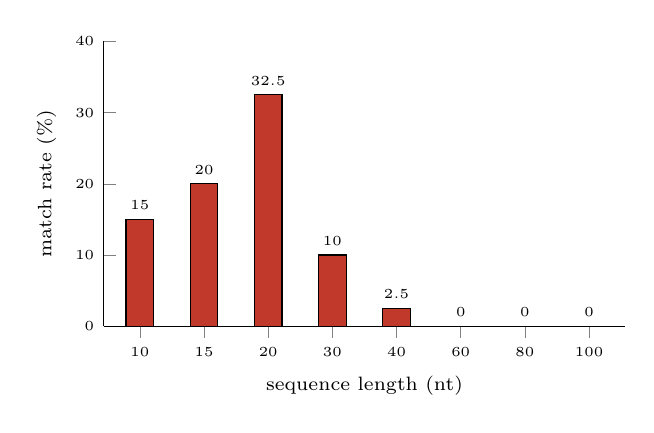
\begin{tikzpicture}
        \begin{axis}[
          width=8.2cm, height=5.2cm,
          ybar, bar width=10pt,
          ymin=0, ymax=40,
          xtick=data, symbolic x coords={10,15,20,30,40,60,80,100},
          xlabel={\scriptsize sequence length (nt)}, ylabel={\scriptsize match rate (\%)},
          nodes near coords, every node near coord/.append style={font=\tiny},
          tick label style={font=\tiny},
          bar shift=0pt,
          axis lines*=left, enlarge x limits=0.08,
        ]
        \addplot[fill=badred] coordinates {(10,15.0) (15,20.0) (20,32.5) (30,10.0) (40,2.5) (60,0.0) (80,0.0) (100,0.0)};
        \end{axis}
      \end{tikzpicture}
      \end{center}
    \end{column}
    \begin{column}{0.36\textwidth}
      \begin{navybox}
      \centering {\color{accent}\huge\textbf{10.0\%}}\\[4pt]
      {\small overall match rate\\ 32 / 320 random sequences}
      \vspace{6pt}\hrule\vspace{6pt}
      \footnotesize 0\% match at $n\geq60$nt --- exactly the length range used in D-Wave scaling runs. Energy gap grows more negative with length: the model doesn't just pick a different fold, it systematically overestimates stability.
      \end{navybox}
    \end{column}
  \end{columns}
\end{frame}

% ============================================================ FINDING: HAIRPIN FIX
\begin{frame}{5. Finding: Real Loop Energies Fix Most of the Gap}
  \small A dynamic program adding real hairpin/bulge/internal-loop energies (via ViennaRNA's own evaluators) on the identical 320-sequence sweep:
  \vspace{4pt}

  \begin{columns}[T]
    \begin{column}{0.62\textwidth}
      \begin{center}
      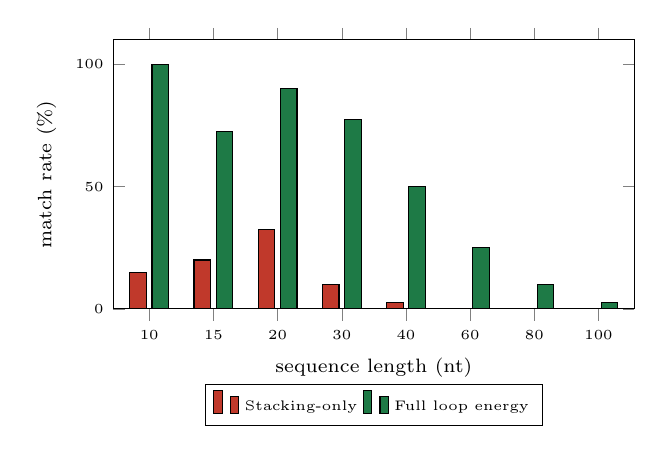
\begin{tikzpicture}
        \begin{axis}[
          width=8.2cm, height=5.0cm,
          ybar, bar width=6pt,
          ymin=0, ymax=110,
          xtick=data, symbolic x coords={10,15,20,30,40,60,80,100},
          xlabel={\scriptsize sequence length (nt)}, ylabel={\scriptsize match rate (\%)},
          tick label style={font=\tiny},
          legend style={font=\tiny, at={(0.5,-0.28)}, anchor=north, legend columns=2},
          enlarge x limits=0.08,
        ]
        \addplot[fill=badred] coordinates {(10,15.0) (15,20.0) (20,32.5) (30,10.0) (40,2.5) (60,0.0) (80,0.0) (100,0.0)};
        \addplot[fill=goodgreen] coordinates {(10,100.0) (15,72.5) (20,90.0) (30,77.5) (40,50.0) (60,25.0) (80,10.0) (100,2.5)};
        \legend{Stacking-only, Full loop energy}
        \end{axis}
      \end{tikzpicture}
      \end{center}
    \end{column}
    \begin{column}{0.36\textwidth}
      \begin{greenbox}
      \centering \textbf{\large 10.0\% $\rightarrow$ 53.4\%}\\[3pt]
      {\footnotesize overall match rate, same 320 sequences}
      \end{greenbox}
      \vspace{6pt}
      \begin{cardbox}
      \textbf{\footnotesize\color{navy}Bug caught mid-build}\\[3pt]
      \tiny A ``free multiloop fallback'' was silently zeroing out hairpin penalties on every closure. Caught by cross-checking against ViennaRNA's own structure evaluator.
      \end{cardbox}
    \end{column}
  \end{columns}
\end{frame}

% ============================================================ DWAVE: EMBEDDING LIMITS
\begin{frame}{6. D-Wave: Embedding Density Limits Direct QPU Use}
  \begin{columns}[T]
    \begin{column}{0.55\textwidth}
      \begin{center}
      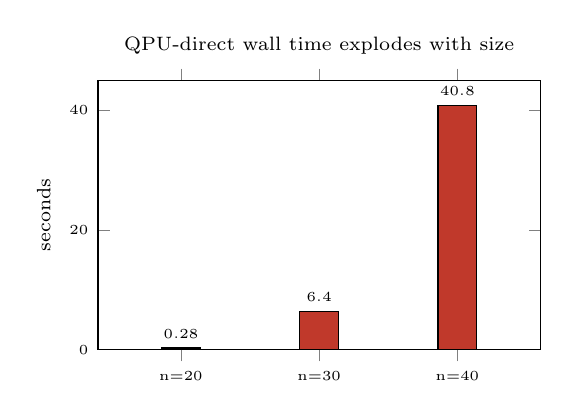
\begin{tikzpicture}
        \begin{axis}[
          width=7.2cm, height=5.0cm,
          ybar, bar width=14pt,
          ymin=0, ymax=45,
          xtick=data, symbolic x coords={n=20,n=30,n=40},
          ylabel={\scriptsize seconds},
          nodes near coords, every node near coord/.append style={font=\tiny},
          tick label style={font=\tiny},
          title={\scriptsize QPU-direct wall time explodes with size},
          enlarge x limits=0.3,
        ]
        \addplot[fill=badred] coordinates {(n=20,0.28) (n=30,6.40) (n=40,40.80)};
        \end{axis}
      \end{tikzpicture}
      \end{center}
      \begin{cardbox}
      \footnotesize\textbf{\color{navy}Meanwhile, actual QPU time stays flat:} 126ms $\rightarrow$ 183ms $\rightarrow$ 125ms (n=20$\to$30$\to$40) --- the escalation above is entirely classical.
      \end{cardbox}
    \end{column}
    \begin{column}{0.42\textwidth}
      \begin{cardbox}
      \textbf{\color{navy}The bottleneck is classical, not quantum}
      \vspace{4pt}
      \begin{itemize}\footnotesize
        \item Constraint graph density stays above 47\% even at 540 variables (100nt) --- far beyond D-Wave's native $\sim$15--20 connections per qubit.
        \item Wall time explodes while actual QPU access time stays essentially constant.
        \item On an identical sequence, direct-QPU solution quality was 39\% worse than hybrid solving ($-11.4$ vs $-18.8$).
      \end{itemize}
      \end{cardbox}
    \end{column}
  \end{columns}
\end{frame}

% ============================================================ DWAVE: HYBRID + CORRECTION
\begin{frame}{7. D-Wave: Hardware Rerun --- Including a Confirmed Correction}
  \small Hairpin-aware rerun on the same 6 sequences. Two already-published results (n=80, n=100) turned out to have exploited a real branching bug --- corrected on real hardware, not silently patched.
  \vspace{4pt}
  \begin{center}
  \small
  \begin{tabular}{lccccc}
    \toprule
    \textbf{n} & \textbf{qubits} & \textbf{qpu\_access ($\mu$s)} & \textbf{energy} & \textbf{feasible} & \textbf{corrected?} \\
    \midrule
    20 & 15 & 109{,}803 & 0.00 & yes & no \\
    30 & 41 & 81{,}754 & $-1.60$ & yes & no \\
    40 & 72 & 91{,}378 & $-5.00$ & yes & no \\
    60 & 178 & 97{,}603 & 0.00 & yes & no \\
    80 & 362 & 150{,}045 & \textbf{\color{badred}$-6.20$ (was $-6.90$)} & yes & \textbf{yes} \\
    100 & 540 & 154{,}952 & \textbf{\color{badred}$-6.70$ (was $-7.93$)} & yes & \textbf{yes} \\
    \bottomrule
  \end{tabular}
  \end{center}
  \vspace{6pt}
  \begin{redbox}
  \footnotesize \textbf{Both wrong values were real hardware output}, not a simulation artifact --- a genuine, previously-undiscovered energy-accounting bug (branching/internal-loop topologies) present in production hardware results already in the repository, found and corrected transparently. Old values preserved, clearly flagged, not deleted.
  \end{redbox}
\end{frame}

% ============================================================ QAOA PENALTY BUG
\begin{frame}{8. QAOA: A Penalty-Landscape Bug --- Fixed, But Not Solved}
  \begin{columns}[T]
    \begin{column}{0.5\textwidth}
      \begin{cardbox}
      \textbf{\color{badred}The problem}\\[5pt]
      \footnotesize The QUBO's classical-exactness penalty ($\approx$2x the sum of every favorable energy) is $\sim$11x larger than any single favorable pairing on small instances.
      \vspace{4pt}

      Irrelevant to a classical exact solver --- but it makes the QAOA landscape so penalty-dominated that ``select nothing, violate nothing'' becomes an inescapable local attractor.
      \vspace{4pt}

      \textit{Confirmed empirically: 0\% match across 8 random restarts, after ruling out insufficient optimizer effort as the cause.}
      \end{cardbox}
    \end{column}
    \begin{column}{0.5\textwidth}
      \begin{greenbox}
      \textbf{\color{accent}The fix (partial)}\\[5pt]
      \footnotesize A much tighter, QAOA-specific penalty ($\sim$1.5x the single largest quartet energy) replaces the classical-exactness penalty for QAOA runs only. Eliminates the total-collapse failure mode above.
      \vspace{4pt}

      \textbf{Does not guarantee success.} A 20-seed sweep found real, measured success rates of only \textbf{15\%} (GGGAAACCC) and \textbf{25\%} (GCGCUUCGGCGC) even on these tiny 4--6 qubit cases --- corrected from an earlier overstated claim after real hardware reruns returned wrong answers.
      \end{greenbox}
    \end{column}
  \end{columns}
\end{frame}

% ============================================================ IBM HARDWARE NOISE WALL
\begin{frame}{9. Real IBM Hardware: Confirmed, Then a Noise Wall}
  \begin{columns}[T]
    \begin{column}{0.5\textwidth}
      \begin{navybox}
      \textbf{\color{accent}4 qubits --- ibm\_kingston}\\[3pt]
      \footnotesize GGGAAACCC: exact match to classical MFE\\[6pt]
      {\Large\textbf{17.0\%}} \quad {\footnotesize shot confidence\\(vs.\ 97.1\% simulator)}
      \end{navybox}
    \end{column}
    \begin{column}{0.5\textwidth}
      \begin{redbox}
      \textbf{6 qubits --- ibm\_marrakesh}\\[3pt]
      \footnotesize GCGCUUCGGCGC: best feasible answer was the trivial empty structure\\[6pt]
      {\Large\textbf{5.2\%}} \quad {\footnotesize shot confidence --- correct answer erased by noise}
      \end{redbox}
    \end{column}
  \end{columns}
  \vspace{8pt}
  \begin{cardbox}
  \textbf{\color{navy}Two more qubits was enough to erase a correct answer entirely}\\[4pt]
  \footnotesize A post-selection bug was also caught here: the plurality bitstring on the 6-qubit run was outright infeasible (malformed structure, energy $\sim$2x the true value). Fixed by ranking all sampled bitstrings by shot count and returning the highest-count feasible one.
  \end{cardbox}
\end{frame}

% ============================================================ IBM ACCESS RESTORED, RERUN
\begin{frame}{9b. IBM Access Restored --- A Correction, Not a Confirmation}
  \small IBM access was reported permanently exhausted earlier in this project. That was wrong --- access was restored, and both toy cases were rerun against the corrected, hairpin-aware QUBO.
  \vspace{6pt}
  \begin{redbox}
  \textbf{Both reruns found the wrong answer on real hardware.}\\[4pt]
  \footnotesize GGGAAACCC $\to$ trivial unfolded structure. GCGCUUCGGCGC $\to$ a different, suboptimal fold. Neither matched the true optimum.
  \end{redbox}
  \vspace{8pt}
  \begin{navybox}
  \textbf{\color{accent}Investigated directly, not dismissed}\\[4pt]
  \footnotesize A 20-seed sweep using the exact hardware-submission parameters found real success rates of only \textbf{15\%} (GGGAAACCC) and \textbf{25\%} (GCGCUUCGGCGC). Today's two hardware failures were the statistically expected outcome ($\sim$64\% combined chance both would fail) --- not a new regression, and not the guaranteed success an earlier version of this deck implied.
  \end{navybox}
  \vspace{8pt}
  \small\textit{This corrected an overstated claim in our own earlier documentation --- caught by the same validate-before-trust discipline used throughout this project.}
\end{frame}

% ============================================================ NOISE STUDY: TWO PLATFORMS
\begin{frame}{10. Noise Study: Two Hardware Platforms, Different Signatures}
  \small D-Wave's noise (chain breaks, annealing) is structurally different from IBM's (gate-based decoherence) --- both characterized, not just one.
  \vspace{6pt}
  \begin{columns}[T]
    \begin{column}{0.48\textwidth}
      \begin{cardbox}
      \textbf{\color{navy}\footnotesize IBM (4 runs, gate-based)}\\[4pt]
      \tiny 3/4 correct across 3 backends. Confidence range for correct answers (17--24\%) overlaps the one incorrect run (15.3\%) --- confidence alone doesn't predict correctness.
      \end{cardbox}
    \end{column}
    \begin{column}{0.48\textwidth}
      \begin{cardbox}
      \textbf{\color{navy}\footnotesize D-Wave (3 runs, annealing)}\\[4pt]
      \tiny All 3 correct, chain-break rate low ($<$7/1000 reads). But read confidence (mean 2.17\%) is 8--10x lower than IBM's --- chain breaks alone don't explain it.
      \end{cardbox}
    \end{column}
  \end{columns}
  \vspace{8pt}
  \begin{navybox}
  \footnotesize Not a clean cross-platform comparison (different qubit counts, different paradigms) --- but each platform shows a genuine, distinct noise signature, honestly characterized rather than conflated into one number.
  \end{navybox}
\end{frame}

% ============================================================ ENCODING COMPARISON
\begin{frame}{11. Comparing Two Quantum Encodings}
  \small Encoding A (quartets, this project) vs.\ Encoding B (raw pairs, prior literature) --- both solve the identical physical model.
  \vspace{4pt}
  \begin{columns}[T]
    \begin{column}{0.55\textwidth}
      \begin{center}
      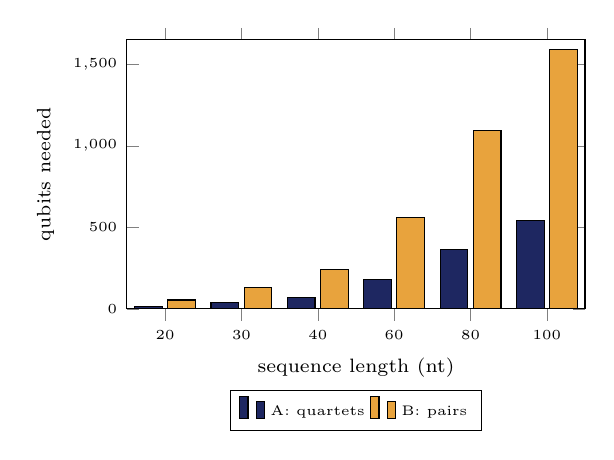
\begin{tikzpicture}
        \begin{axis}[
          width=7.4cm, height=5.0cm,
          ybar, bar width=10pt,
          ymin=0, ymax=1650,
          xtick=data, symbolic x coords={20,30,40,60,80,100},
          xlabel={\scriptsize sequence length (nt)}, ylabel={\scriptsize qubits needed},
          tick label style={font=\tiny},
          legend style={font=\tiny, at={(0.5,-0.3)}, anchor=north, legend columns=2},
          enlarge x limits=0.1,
        ]
        \addplot[fill=navy] coordinates {(20,15) (30,41) (40,72) (60,178) (80,362) (100,540)};
        \addplot[fill=accent] coordinates {(20,55) (30,130) (40,239) (60,560) (80,1093) (100,1590)};
        \legend{A: quartets, B: pairs}
        \end{axis}
      \end{tikzpicture}
      \end{center}
    \end{column}
    \begin{column}{0.42\textwidth}
      \begin{navybox}
      \textbf{\large $\sim$3x more qubits}\\[3pt]
      \footnotesize Encoding B consistently needs $\sim$3x more qubits than Encoding A (ratio 2.94--3.67), but has a less dense constraint graph.
      \end{navybox}
      \vspace{6pt}
      \begin{cardbox}
      \footnotesize\textbf{\color{navy}Degenerate optimum, verified:} at n=20, both encodings found different structures tied at the exact same optimal energy ($-5.00$) --- confirmed independently, not a bug.
      \end{cardbox}
    \end{column}
  \end{columns}
\end{frame}

% ============================================================ PSEUDOKNOTS
\begin{frame}{12. Pseudoknots: A Validated Proof-of-Concept}
  \small Not general pseudoknot folding (NP-hard) --- relaxed the no-crossing constraint and proved the solver correctly exploits it when genuinely favorable.
  \vspace{6pt}
  \begin{columns}[T]
    \begin{column}{0.5\textwidth}
      \begin{cardbox}
      \textbf{\color{navy}\footnotesize Hand-verified test case}\\[4pt]
      \tiny 26nt sequence, two independent 5bp stems designed to cross. Verified programmatically: both canonical, outer pairs $(0,19)$ and $(7,25)$ provably cross.
      \end{cardbox}
    \end{column}
    \begin{column}{0.5\textwidth}
      \begin{cardbox}
      \small
      \begin{tabular}{@{}lr@{}}
        Non-crossing baseline & $-8.70$ \\
        Pseudoknot-permissive & \textbf{$-17.40$} \\
      \end{tabular}\\[4pt]
      \tiny Exactly matches hand-calculated expectation. Independently re-verified: no base reused, all pairs canonical, energy recomputed from scratch matches exactly.
      \end{cardbox}
    \end{column}
  \end{columns}
  \vspace{8pt}
  \begin{navybox}
  \footnotesize \textbf{Honest scope:} no real pseudoknot-specific loop-topology penalties (Rivas \& Eddy terms) --- crossing quartets scored identically to nested ones. A real, stated simplification, not hidden.
  \end{navybox}
\end{frame}

% ============================================================ LIMITATIONS
\begin{frame}{13. Limitations}
  \begin{columns}[T]
    \begin{column}{0.5\textwidth}
      \begin{cardbox}
      \textbf{\footnotesize\color{badred}No multiloop support}\\[3pt]
      \tiny Neither the DP nor the QUBO models multi-branch loops. Scoped out, not hidden.
      \end{cardbox}
      \vspace{4pt}
      \begin{cardbox}
      \textbf{\footnotesize\color{badred}QUBO still lacks bulge/internal loops}\\[3pt]
      \tiny DP proves full model works (10.0\%$\to$53.4\%); porting to the QUBO is the single biggest remaining gap.
      \end{cardbox}
      \vspace{4pt}
      \begin{cardbox}
      \textbf{\footnotesize\color{badred}No pseudoknot energy penalties}\\[3pt]
      \tiny Crossing quartets scored the same as nested ones --- a real simplification.
      \end{cardbox}
    \end{column}
    \begin{column}{0.5\textwidth}
      \begin{cardbox}
      \textbf{\footnotesize\color{badred}QAOA succeeds only 15--25\% of the time}\\[3pt]
      \tiny Measured directly via a 20-seed sweep on toy cases. Model confirmed correct via simulated annealing --- the landscape is genuinely harder for a shallow circuit, not a bug.
      \end{cardbox}
      \vspace{4pt}
      \begin{cardbox}
      \textbf{\footnotesize\color{badred}IBM hardware noise dominates by 6 qubits}\\[3pt]
      \tiny On the current backend/circuit combination, without deeper error mitigation.
      \end{cardbox}
      \vspace{4pt}
      \begin{cardbox}
      \textbf{\footnotesize\color{badred}D-Wave's n=100 QPU trigger unexplained}\\[3pt]
      \tiny Only 1 of 6 sequences invoked the QPU at all; the connected-components hypothesis was tested and refuted, real cause still unconfirmed.
      \end{cardbox}
    \end{column}
  \end{columns}
\end{frame}

% ============================================================ FUTURE WORK
\begin{frame}{14. Future Work}
  \begin{enumerate}\small
    \item Port bulge/internal-loop energies into the QUBO --- proven worthwhile by the DP, highest-priority remaining gap.
    \item Proper multiloop DP and QUBO extension (WM table, branch counting).
    \item Diagnose and fix QAOA's difficulty with the hairpin-aware Hamiltonian's correlated landscape.
    \item Real pseudoknot-specific energy penalties (Rivas \& Eddy terms) and a systematic scan across random sequences.
    \item Error mitigation to push usable QAOA qubit count past the observed noise wall.
    \item Extend the D-Wave noise study to more qubit counts using the newly-added chain-break/confidence metrics.
    \item Investigate D-Wave's apparent size-based QPU-access threshold directly.
  \end{enumerate}
\end{frame}

% ============================================================ CLOSING
{
\setbeamertemplate{footline}{}
\begin{frame}[plain]
  \begin{tikzpicture}[remember picture, overlay]
    \fill[navy] (current page.south west) rectangle (current page.north east);
  \end{tikzpicture}
  \vspace{1.6cm}
  {\color{white}\Huge\textbf{Thank you}\par}
  \vspace{0.6cm}
  {\color{ice}\large Every finding in this deck came from checking a plausible-looking result against\\ independent ground truth --- including corrections to our own published results.\par}
  \vspace{0.6cm}
  {\color{accent}\rule{3.5cm}{1.5pt}\par}
  \vspace{0.4cm}
  {\color{white}\large \texttt{github.com/Qyngshuk08/wiser-2026-moderna-challenge}\par}
  {\color{muted}\large Team Qudit Creons \; $\vert$ \; WISER 2026 --- Moderna Challenge\par}
\end{frame}
}

\end{document}
